Для оценки качества работы алгоритма, следуя работе \cite{Romanenko2012}, будем измерять качество одноклассовой класификации в терминах точности и полноты.
В нашем случае точность (precision, $P$)~--- доля верно классифицированных объектов тестовой выборки среди всех объектов, отнесенных алгоритмом к единственному классу.
Полнота (recall, $R$)~--- доля верно классифицированных объектов тестовой выборки среди всех объектов, принадлежащих к единственному классу.
Более высокие значения точности и полноты соответствуют лучшему качеству классификации.
В качестве агрегированного показателя, объединяющего точность $P$ и полноту $R$ используем $F_1$-меру \cite{Rijsbergen1979}:
$$F_1 = \frac{2PR}{P+R}.$$
%Большим значениям $P$ и $R$ соотвтествую

Для проведения вычислительного эксперимента\footnote{Код доступен по адресу \textsf{https://github.com/burmisha/daml/tree/master/9\_term/aspam}} на модельных данных
сгенерируем $N=400$ случайных точек $\fbr{\mb x_i}_{i=1}^N$ из распределения (\ref{PhiXARC}) 
при размерности пространства $n=2$ (для наглядности), положив направления смещений случайными и придав параметрам значения $\mb a = \cbr{1,2}\T, R = 3, c = 0{,}2.$
После этого проведем $t{\times}q$-fold кросс-валидацию с $t = 10, q = 3$, скользящим контролем подбирая параметр $C$ по значению $F_1$-метрики.
При вычислении $F_1$-метрики все объекты, лежащие вне построенной сферы с центром $\hat{\mb a}$ и радиуса $\hat R$, мы считаем не принадлежащим классу, 
а все объекты внутри неё~--- считаем, поскольку нашей задачей является именно поиск этой гиперсферы.

На рисунке \ref{tikz:CV} изображена полученная зависимость значения $F_1$-метрики от параметра $C$.
Из графика видно, что при $C\to 0$ обобщающая способность стремится к нулю, поскольку практически отсутствует штраф за непопадание в класс при обучении.
При этом большие штрафы заставляют необоснованно увеличивать сферу, снижая точность.

Пример работы алгоритма приведен на рисунке \ref{tikz:workexample} при параметрах $n=2, N=400, R=3, \mb a = \cbr{1,2}\T, c=0{,}6, C = 0{,}007.$ Здесь 2-мерная сфера строилась по всем $N$ объектам.
Зеленым изображена граница истинного распределения, красным~--- построенного.
Видно, что здесь $C$ оказалось слишком мало и сфера получилось описывает лишь небольшую часть объектов.

\begin{figure}[h]
	\centering
	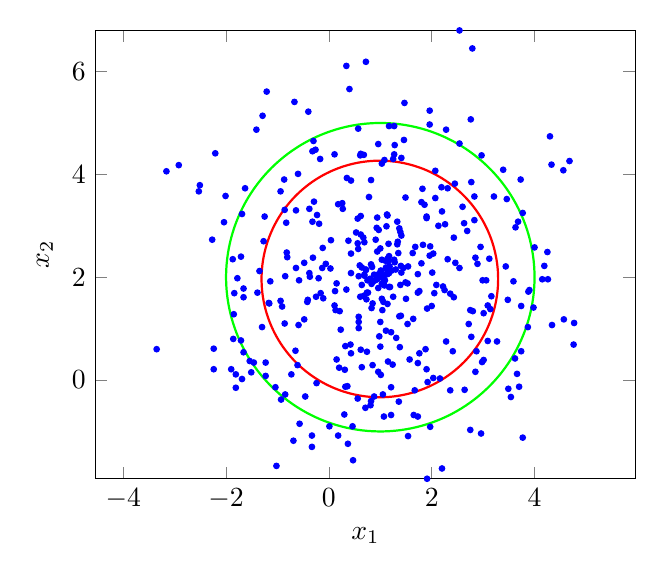
\begin{tikzpicture}
		\begin{axis}[xlabel=$x_1$, ylabel=$x_2$, enlargelimits=false, scaled ticks=false,axis equal=true]
			\addplot +[green, mark=none, domain=0:360,samples=180, thick]({1 + 3*cos(x)},{2+3*sin(x)});
			\addplot [blue, only marks, mark size=1pt]  coordinates {
			 (3.62,0.42)(-1.30,1.03)(0.12,1.73)(2.20,3.28)(-0.41,1.56)(0.36,-0.12)(-1.04,-0.14)(0.64,1.85)(-1.66,0.54)(-1.51,0.15)(-0.25,1.62)(0.43,0.52)(-0.83,3.06)(2.36,-0.20)(-1.71,2.40)(3.63,2.97)(0.42,0.69)(-0.58,1.94)(-2.53,3.67)(2.77,0.84)(4.15,1.96)(1.37,2.95)(1.67,-0.20)(2.31,3.73)(-2.21,4.41)(0.72,2.15)(-0.85,2.02)(0.31,0.20)(1.30,2.15)(2.75,-0.97)(3.73,3.90)(1.49,3.55)(-1.87,2.35)(1.53,1.88)(2.16,0.03)(0.58,1.13)(1.86,3.41)(1.96,4.97)(1.33,2.64)(2.03,2.46)(0.64,0.25)(0.62,3.19)(1.27,4.94)(-3.35,0.60)(1.35,2.47)(1.00,1.13)(3.27,0.75)(-0.38,2.08)(-1.02,-1.67)(0.34,6.11)(-1.27,2.70)(4.19,2.22)(1.90,3.18)(2.07,4.07)(-2.92,4.18)(-0.86,1.10)(4.57,1.18)(-0.87,3.90)(2.28,0.75)(2.87,0.56)(-1.69,0.02)(1.73,2.06)(1.90,3.15)(2.79,6.45)(2.43,1.61)(3.09,0.76)(1.47,5.39)(2.54,6.80)(2.83,3.57)(0.74,1.70)(1.03,1.87)(1.08,4.28)(-0.64,3.30)(4.33,4.19)(1.65,-0.68)(3.44,2.21)(0.20,0.24)(1.39,2.88)(4.76,0.69)(2.99,1.94)(1.07,1.92)(-0.60,4.01)(2.69,2.90)(0.83,1.87)(-0.33,-1.08)(1.31,0.82)(1.80,2.27)(1.41,2.09)(0.98,0.85)(1.37,1.24)(-1.39,1.70)(1.17,2.18)(2.01,2.09)(1.11,0.96)(0.37,-1.24)(0.18,3.42)(3.74,1.44)(3.14,1.38)(3.46,3.52)(1.03,1.58)(4.30,4.74)(-1.63,3.73)(1.17,2.08)(0.85,0.29)(0.04,2.72)(2.45,3.82)(1.40,1.25)(2.83,3.11)(-1.17,1.50)(2.03,0.04)(1.88,0.60)(0.88,2.05)(0.82,3.89)(0.32,0.66)(1.28,2.29)(-0.48,1.18)(1.80,3.46)(2.95,2.59)(-1.71,0.77)(0.96,4.59)(4.26,1.96)(1.14,2.13)(1.76,1.73)(1.57,0.40)(-2.51,3.79)(0.57,4.89)(1.76,0.52)(2.22,1.82)(1.11,2.19)(-0.46,-0.32)(2.07,3.54)(0.91,2.73)(-0.19,3.04)(0.83,1.40)(-1.78,1.98)(-0.31,2.38)(-1.41,4.87)(0.97,2.06)(1.97,-0.91)(1.25,4.30)(-0.94,1.54)(0.56,-0.36)(1.21,-0.68)(1.16,2.31)(4.25,2.49)(1.03,2.04)(-0.06,2.26)(1.16,2.65)(0.47,-1.56)(0.75,1.94)(-1.14,1.92)(-1.35,2.12)(0.61,4.37)(-2.04,3.07)(0.80,1.97)(2.54,4.60)(-0.29,3.47)(-0.73,0.11)(1.63,2.47)(1.90,0.21)(3.59,1.92)(2.20,-1.72)(1.15,0.36)(0.72,2.14)(0.96,1.79)(0.88,-0.32)(-1.23,0.08)(0.71,-0.54)(2.25,1.75)(-0.67,5.41)(2.80,1.34)(4.77,1.11)(1.19,1.81)(1.34,2.69)(-1.84,1.69)(-0.40,5.22)(3.68,3.08)(1.91,1.39)(1.00,2.56)(2.28,4.87)(3.88,1.72)(1.12,2.99)(0.67,2.77)(-0.11,1.59)(-0.93,-0.38)(3.77,3.25)(2.60,3.37)(2.19,3.75)(1.53,1.09)(-0.17,4.30)(1.17,4.94)(2.26,3.03)(-0.64,2.18)(1.24,0.30)(1.64,1.19)(0.81,-0.49)(3.70,-0.13)(4.34,1.07)(0.30,-0.67)(0.93,2.96)(0.11,4.39)(1.06,1.52)(1.25,1.62)(0.34,1.76)(1.14,1.48)(3.09,1.45)(1.18,2.21)(3.98,1.41)(-1.66,1.78)(-0.69,-1.18)(1.73,0.33)(0.82,-0.41)(-2.27,2.73)(-0.91,1.43)(1.83,2.63)(-1.21,5.61)(1.12,2.06)(-0.20,1.98)(3.77,-1.12)(1.00,0.65)(-0.13,2.18)(1.17,2.41)(-2.24,0.61)(1.49,1.90)(1.13,3.22)(-2.01,3.58)(-0.59,1.07)(-0.86,3.31)(3.12,2.36)(2.98,0.35)(1.01,2.11)(2.72,1.09)(0.90,1.94)(4.00,2.58)(-0.12,2.57)(1.54,-1.09)(0.62,2.83)(1.21,-0.14)(-2.24,0.21)(1.08,1.84)(1.14,2.14)(1.07,1.97)(3.48,1.56)(1.03,4.21)(0.58,2.02)(-1.85,1.28)(1.05,-0.28)(1.17,1.81)(1.22,2.13)(0.73,1.57)(3.90,1.75)(1.03,2.34)(0.58,1.23)(1.68,2.59)(1.14,2.36)(0.18,-1.08)(3.01,0.39)(3.21,3.57)(0.68,4.38)(1.82,3.72)(1.14,3.20)(1.36,-0.42)(1.27,2.34)(0.61,1.62)(0.94,1.96)(1.91,-1.92)(4.56,4.08)(0.60,2.23)(-0.23,3.21)(0.62,4.40)(0.58,1.01)(-0.26,4.48)(3.06,1.94)(0.78,3.56)(0.53,2.87)(-0.32,4.45)(-1.90,0.21)(-1.66,1.61)(-0.48,2.28)(0.40,5.66)(0.38,2.71)(0.43,3.88)(-1.29,5.14)(0.03,2.17)(0.97,2.92)(2.96,-1.04)(0.84,2.20)(2.09,1.85)(-0.65,0.57)(0.69,2.68)(-0.61,0.29)(0.46,-0.90)(-0.81,2.39)(-0.24,-0.06)(-0.85,-0.28)(0.15,1.88)(-1.16,1.49)(1.39,1.85)(2.89,2.26)(3.74,0.56)(-0.33,-1.30)(0.96,0.16)(0.21,1.34)(1.27,4.39)(-1.81,-0.15)(-0.82,2.48)(0.72,6.19)(0.43,2.46)(0.64,2.19)(2.05,1.69)(0.62,0.59)(2.54,2.18)(2.00,1.44)(-0.94,3.67)(1.10,2.32)(2.46,2.28)(1.21,0.93)(1.33,3.08)(0.76,1.70)(3.16,1.63)(0.11,1.45)(0.43,2.08)(1.00,2.00)(1.96,2.42)(0.35,3.93)(-0.57,-0.85)(1.14,2.06)(3.54,-0.33)(1.45,2.18)(2.97,4.37)(-0.30,4.65)(2.76,5.07)(0.94,2.50)(2.75,1.36)(-0.42,1.52)(1.04,1.36)(3.01,1.30)(0.32,-0.13)(0.56,2.66)(-0.38,3.33)(-3.16,4.06)(0.15,0.40)(2.77,3.85)(0.27,3.33)(1.01,2.13)(0.13,1.36)(-1.69,3.23)(0.23,0.98)(0.82,2.25)(2.85,2.38)(2.31,2.35)(2.64,-0.19)(2.63,3.05)(-1.46,0.34)(-1.54,0.37)(0.57,2.55)(1.40,2.22)(3.87,1.03)(1.41,4.32)(0.99,2.06)(-1.81,0.11)(1.01,0.10)(2.41,0.56)(1.92,-0.04)(1.73,-0.71)(3.39,4.09)(1.38,0.64)(0.69,2.05)(1.07,-0.71)(0.56,3.14)(-1.86,0.80)(-0.37,2.01)(0.01,-0.90)(1.50,1.58)(0.68,1.64)(3.49,-0.17)(0.86,1.92)(-1.25,3.18)(1.46,4.67)(0.26,3.44)(2.36,1.68)(4.68,4.26)(0.74,0.55)(2.43,2.77)(1.54,2.21)(-0.16,1.69)(0.94,3.16)(1.96,5.24)(1.41,2.81)(1.97,2.60)(2.13,3.00)(2.85,0.16)(0.85,1.49)(3.66,0.12)(0.69,2.03)(-0.32,3.08)(1.09,1.94)(-1.23,0.34)(1.28,4.57)(1.73,1.70)
		};
		\addplot+[red,  mark=none, domain=0:360,samples=180, thick]({0.9909 + 2.3010*cos(x)},{1.9660+2.3010*sin(x)});
		\end{axis}
	\end{tikzpicture}
	\caption{Пример результата работы алгоритма при $C = 0{,}007.$}
	\label{tikz:workexample}
\end{figure}

Примеры работы алгоритма при использовании ядер приведены на рисунках \ref{eps:example_rbf_1}, \ref{eps:example_rbf_10}. 
Зеленые круги~--- смесь трёх распределений с общим $R = 1{,}5, c = 0{,}6$ и различными центрами: 
\begin{itemize}
	\item $\mb a_1 = 			(1,6)\T, N_1 = 150$,
	\item $\mb a_2 = \mb a_1 + 	(5,0)\T, N_2 = 75$,
	\item $\mb a_3 = \mb a_1 + 	(3,4)\T, N_3 = 50$.
\end{itemize}
Значение гиперпараметра положено равным $C = 0{,}015$. Синим отмечена построенная разделяющая поверхность. Существенной проблемой подхода является вопрос связности построенных областей: например, встречаются области, не отнесенные алгоритмом к классу, полностью содержащиеся в областях, которые алгоритм принял за относящиеся.
\addeps{example_rbf_1}{РБФ Гаусса: $C = 0{,}015, s=1.$}
\addeps{example_rbf_10}{РБФ Гаусса: $C = 0{,}015, s=10.$}

Эксперимент на реальных данных был проведен с использованием данных, находящихся в открытом доступе\footnote{UCI Machine Learning Repository \textsf{http://archive.ics.uci.edu/ml/datasets/Spambase}}. 
Эти данные содержат уже вычисленные признаки сообщений.
Использованная база в себе как объекты, относящиеся к спаму, так и не относящиеся.
Каждый из $n = 57$ признаков документов линейно отображался в отрезок $[0, 1]$, чтобы учесть различие в их масштабах. 
Для обучения бралась небольшая часть спам-документов (200 из ~1800).
Затем по новым точкам ним строилась сфера (в 57-мерном пространстве).

В эксперименте контрольная выборка содержала все доступные объекты (в том числе объекты из обучения). 
Для каждого из объектов контрольной выборки проверялось попадание в построенную сферу и далее вычислялась $F_1$-метрика.
Отдельно стоит отметить, что в контроле участвуют как объекты из исследуемого класса (спам-сообщений), так и не из него, хотя обучение происходило только на объектах целевого класса (спама).
Результаты подбора параметра $C$ изображены на рисунке (\ref{tikz:CV}). Данные усреднены по 20 случайным выборкам без повторений по 200 объектов из 1800.

\begin{figure}[h]
	\begin{minipage}[h]{0.5\linewidth}
		\centering % Model_N400_0.0150-0.0005-0.0450_T20_Q3
		\begin{tikzpicture}%[x=3cm,y=3cm]
			\begin{axis}[xlabel=$C$, ylabel=$F_1$, enlargelimits=false,title={Модельные данные},
			scaled x ticks=false,xticklabel style={/pgf/number format/fixed, /pgf/number format/precision=3}]
			%_CV_Model_N400_0.0150-0.0005-0.0450_T20_Q3
			\addplot[red, mark=none, thick] coordinates {
				(0.0150, 0.9302)(0.0155, 0.9363)(0.0160, 0.9388)(0.0165, 0.9435)(0.0170, 0.9447)(0.0175, 0.9451)(0.0180, 0.9474)(0.0185, 0.9506)(0.0190, 0.9513)(0.0195, 0.9567)(0.0200, 0.9590)(0.0205, 0.9617)(0.0210, 0.9653)(0.0215, 0.9673)(0.0220, 0.9710)(0.0225, 0.9734)(0.0230, 0.9767)(0.0235, 0.9775)(0.0240, 0.9780)(0.0245, 0.9785)(0.0250, 0.9819)(0.0255, 0.9833)(0.0260, 0.9816)(0.0265, 0.9823)(0.0270, 0.9841)(0.0275, 0.9837)(0.0280, 0.9852)(0.0285, 0.9836)(0.0290, 0.9842)(0.0295, 0.9841)(0.0300, 0.9836)(0.0305, 0.9827)(0.0310, 0.9823)(0.0315, 0.9826)(0.0320, 0.9831)(0.0325, 0.9818)(0.0330, 0.9813)(0.0335, 0.9812)(0.0340, 0.9831)(0.0345, 0.9830)(0.0350, 0.9819)(0.0355, 0.9825)(0.0360, 0.9825)(0.0365, 0.9809)(0.0370, 0.9810)(0.0375, 0.9785)(0.0380, 0.9806)(0.0385, 0.9805)(0.0390, 0.9805)(0.0395, 0.9806)(0.0400, 0.9806)(0.0405, 0.9802)(0.0410, 0.9805)(0.0415, 0.9797)(0.0420, 0.9789)(0.0425, 0.9782)(0.0430, 0.9795)(0.0435, 0.9779)(0.0440, 0.9781)(0.0445, 0.9783)(0.0450, 0.9782)
			};
			%\legend{$\ln Iter$, $\ln n!$}
			\end{axis}
		\end{tikzpicture}
  	\end{minipage}
	\hfill
  	\begin{minipage}[h]{0.5\linewidth}
		\centering
		\begin{tikzpicture}%[x=3cm,y=3cm]
			\begin{axis}[xlabel=$\mu$, ylabel=$S$, title={Реальные данные},
						 scaled ticks=false, enlargelimits=false,
						 xticklabel style={/pgf/number format/fixed, /pgf/number format/precision=1},
						 yticklabel style={/pgf/number format/fixed, /pgf/number format/precision=5}
						]
			\addplot[red, mark=none, thick] coordinates {
				
			};
			\end{axis}
		\end{tikzpicture}
	\end{minipage}
	\caption{Зависимость $F_1$-метрики от параметра регуляризации $C$}
	\label{tikz:CV}
\end{figure}

% \addeps{CrValLong}{Модельные данные. Зависимость $F_1$-метрики от параметра регуляризации $C$.}  % CV_0.000-0.010-0.200_T10_Q3.eps
% \addeps{example}{Пример результата работы алгоритма при $C = 0{,}007.$}

В обоих экспериментах отчетливо прослеживаются максимумы метрики, что свидетельствует о наличии в обеих задачах оптимального значения параметра $C.$

Результат, полученный при использовании ядра Гаусса, изображен на рисунке \ref{tikz:CV_rbf}. Ещё раз отметим, что отличие заключается лишь в записи задачи квадратичной оптимизации: теперь вместо скалярного произведения следует вычислять значения ядерной функции. Использовался параметр $s=0{,}7$, при этом при его вариации значения $F_1$-метрики менялись незначительно.

\begin{figure}[h]
	\centering 
	\begin{tikzpicture}%[x=3cm,y=3cm]
		\begin{axis}[xlabel=$C$, ylabel=$F_1$, title={Реальные данные},
					 scaled ticks=false, enlargelimits=false,
					 xticklabel style={/pgf/number format/fixed, /pgf/number format/precision=3},
					 yticklabel style={/pgf/number format/fixed, /pgf/number format/precision=3}
					]
			%_CV_Real_N300_0.0400-0.0040-0.1200_T20_rbf0.700
			\addplot[red, mark=none, thick] coordinates {
				(0.040,0.7450)(0.044,0.7443)(0.048,0.7475)(0.052,0.7465)(0.056,0.7468)(0.060,0.7469)(0.064,0.7463)(0.068,0.7482)(0.072,0.7480)(0.076,0.7489)(0.080,0.7439)(0.084,0.7487)(0.088,0.7462)(0.092,0.7439)(0.096,0.7485)(0.100,0.7480)(0.104,0.7481)(0.108,0.7469)(0.112,0.7486)(0.116,0.7464)(0.120,0.7469)
			};
		\end{axis}
	\end{tikzpicture}
	\caption{Зависимость $F_1$-метрики от $C$ при РБФ Гаусса с $s = 0.7$}
	\label{tikz:CV_rbf}
\end{figure}

Видно, что результаты не столь устойчивы, однако они стабильно выше результатов обычного алгоритма в достаточно широком диапазоне параметра регуляризации. Этот факт позволяет судить об эффективности предложенного подхода.
